\documentclass[11pt]{article}
% packages
\usepackage[utf8]{inputenc}
\usepackage{geometry}
\usepackage[pdftex]{graphicx}
\usepackage{tabularx}
\usepackage{dsfont}
\usepackage{multirow}
\usepackage{amsmath,amsfonts,amssymb}
\usepackage{subcaption}
\usepackage{authblk}
\usepackage{placeins}
%hyperlinks options
\usepackage{hyperref}
\hypersetup{colorlinks=true,linkcolor=blue,filecolor=magenta,urlcolor=cyan,citecolor=cyan}
%bib options
\usepackage[backend=biber,style=authoryear,bibstyle=authoryear,natbib=true,
giveninits=true,uniquename=false,uniquelist=false,% firstinits=false,
maxcitenames=2,date=year, maxbibnames=99,url=false]{biblatex}
\geometry{left=20mm, top=20mm, right=20mm}
%float barrier
\usepackage{placeins}
 \addbibresource{Thèse.bib}
\title{Chapitre 3 : Analyse probabiliste des crues du XVI\textsuperscript{ème} siècle à aujourd'hui}
\author{Mathieu}


\begin{document}
\maketitle

\tableofcontents

\section{Introduction du chapitre}
	Quelques rappels d'intro aux méthodes d'analyse des crues histo:
	\cite{stedinger_flood_1986}\\
	Solutions quand le débit est connu\\
	Solution quand le débit n'est pas connu	\\
%	plot positions (\citet{hirsch_techniques_1982}...)	\\
	Explication du concept de seuil de perception et de ses limites.\\
	durée de la période historique\\
	
	\paragraph{Méconnaissance du seuil}
	Le seuil de perception est un concept empirique qui ne prend une signification physique que dans certaines situations. Par exemple, imaginons une station hydrométrique dont la section n'a pas évolué au cours du temps et pour laquelle les débordements surviennent toujours au delà d'un même débit. Ces débordements (par exemple au-dessus d'une digue qui n'a subi aucune modification au cours du temps) laissent systématiquement une trace dans les écrits ou sur des infrastructures (marques de crue) suite aux dommages occasionnés. Cette situation parfaite existe rarement et le concept de seuil de perception peut être mis à mal par une variabilité temporelle de la perception des crues par les populations ripariennes. Néanmoins, l'utilisation du concept de seuil de perception est très souvent obligatoire pour exploiter les données de crues historiques. 
	
	\paragraph{Méconnaissance de la durée histo}Cette durée est pourtant importante dans le calcul de la binomiale. Il est erroné de considérer que la période historique démarre à la première crue et cela peut entrainer une sur-estimation de la fréquence d'occurrence. Plusieurs méthodes existent dans la littérature pour calculer cette durée et se basent sur (A COMPLETER...). 
		
\section{Méthodes d'analyse probabiliste d'un échantillon mixte de crues}
	
	
	\subsection{Concepts de base et hypothèses}
	
	\paragraph{} 
	
		L'utilisation d'occurrences de crues historiques pour l'analyse fréquentielle nécessite a minima l'hypothèse suivante : le débit de tous les événements de crue qui ont laissé une trace est supérieur à un seuil de perception. Il existe des méthodes d'analyse pour lesquelles il n'est pas nécessaire de connaitre précisément le débit de ces événements (voir notamment \citet{stedinger_flood_1986}). Le nombre de dépassements d'un seuil de perception pour une durée donnée est une information qui peut être exploitée en l'état. Ainsi, il faut considérer un échantillon mixte, composé d'une part de débits enregistrés en continu et d'autre part d'un nombre d'occurrences de crues supérieures à un seuil de perception. 
			
		\paragraph{}
		De manière similaire au Chapitre 1 (REF), on suppose que le débit maximum annuel des périodes continues et historiques $Q$ est une variable aléatoire $iid$ qui suit une distribution GEV, de paramètres $\boldsymbol{\theta} = (\mu,\sigma,\xi)$ (respectivement : position, échelle, forme). Pour simplifier, on suppose ici que le paramètre de forme $\xi$ est différent de zéro (forme Gumbel). Ainsi, on a la fonction de répartition de la GEV : $F(x;\boldsymbol{\theta}) = e^{-(1-\xi(\frac{x - \mu}{\sigma}))^{1/\xi}}$. Les débits de l'échantillon de maximum annuels enregistrés en continu pendant $j$ années $\boldsymbol{q}= (q_t)_{t=1,...,j}$ sont ici supposés parfaitement connus et ne sont donc pas affectés de quelconque incertitude. L'échantillon historique est composé de $k$ événements ayant dépassé le seuil de perception $S$ sur une période de $n$ années. Le seuil de perception n'a donc pas été dépassé pour les $k-n$ années restantes. Ainsi, la probabilité de dépassement du seuil peut s'écrire :
		
		\begin{equation}
			\pi = \biggl( 1 - F(S;\boldsymbol{\theta})\biggl) = 1 - e^{-\biggl(1-\xi\bigl(\frac{S-\mu}{\sigma}\bigl)\biggl)^{1/\xi} }		
		\end{equation}
			 
	On suppose que $k$, le nombre de dépassements du seuil de perception, peut être estimé par une loi binomiale de paramètres $n$ et $\pi$, soit $\mathcal{B}(n,\pi)$. On peut alors écrire la fonction de vraisemblance suivante (\ref{eq:Gev_Binom}) qui est fonction d'un échantillon mixte de données composé des débits maximum annuels de la période continue $(q_t)_{t=1,...,j}$ et du nombre de dépassement du seuil durant la période historique $k$.
		
			\begin{equation}
			L(\boldsymbol{\theta} ; \boldsymbol{q}, k) = \underbrace{\prod_{t=1}^j f\left(q_t;\boldsymbol{\theta}\right)}_{\mathrm{a}} \underbrace{\left\{\left(\begin{array}{l}
			n \\
			k
			\end{array}\right) F\left(S;\boldsymbol{\theta}\right)^{n-k}\left[1-F\left(S;\boldsymbol{\theta}\right)\right]^k\right\}}_{\mathrm{b}} \\
			\label{eq:Gev_Binom}
			\end{equation}
			
			Ici, le terme $a$ représente la vraisemblance pour les données continues et le terme $b$ pour les données historiques. L'application de la formule de Bayes permet de calculer la distribution a posteriori des paramètres $\boldsymbol{\theta}$ sachant les données :
			
			\begin{equation}
				P(\boldsymbol{\theta} \mid \boldsymbol{q},k) \propto L(\boldsymbol{\theta};\,\boldsymbol{q},k) P(\boldsymbol{\theta})
				\label{eq:BayesBinom}
			\end{equation}
	
		Le terme $P(\boldsymbol{\theta})$ représente ici la distribution a priori des paramètres qu'il faudra éliciter. La distribution a posteriori est explorée via une méthode Bayésienne MCMC (notamment décrites par \citet{coles_classical_2001}). Cette distribution a posteriori représente l'incertitude d'échantillonnage du modèle par $r$ jeux de paramètres : $\boldsymbol{\Theta} = (\boldsymbol{\theta_1},...,\boldsymbol{\theta_r})$. Le jeu de paramètres le plus probable est appelé maxpost et s'écrit $\boldsymbol{ \hat{\theta} }$.
	
	
%	\paragraph{Description difficultés de détermination du seuil et durée historique}
%	Complexité de déterminer le seuil\\
%	Complexité de déterminer la durée de la période historique \citep{prosdocimi_german_2018}). 			Attention aux confusions entre date de début de la période et durée de la période. \\

	
	\subsection{Propagation des incertitudes hydrométriques de la période continue}
	
	\paragraph{}
	Dans la section précédente, l'incertitude autour des débits maximum annuels de la période continue est supposée négligeable. Cette incertitude pouvant atteindre 30 \% à Beaucaire (REF Chap 1), il semble pragmatique de la considérer. Comme décrit dans la section REF du Chapitre 1, cette incertitude hydrométrique est représentée par $s = 500$ réalisations : $(q_t^{(i)})_{t=1,...,j;\,i=1,...,s}$. Elle peut être propagée aux estimations des paramètres de l'équation \ref{eq:Gev_Binom} en estimant un jeu de paramètres pour chacune des $s$ réalisations, soit $(\boldsymbol{\theta}
	^{(i)})_{i=1,...,s}$. Au total, $r \times s$ jeux de paramètres sont estimés et représentent l'effet combiné de l'incertitude d'échantillonnage et de l'incertitude hydrométrique des données continues, on a donc $(\boldsymbol{\theta}^{(i)}_p)_{p=1,...,r;\, i=1,...,s}$. Le jeu de paramètres le plus probable est calculé en utilisant l'échantillon maxpost de débits maximum annuels (CHAPITRE 1) sur lequel on estime le jeu de paramètres maxpost de l'équation \ref{eq:Gev_Binom}. Ce modèle sera appelé "modèle A". La propagation des incertitudes hydrométriques de la période continue telle que décrite ici est également effectuée pour les trois modèles définis dans les sections suivantes.
	
	\subsection{Incertitudes autour du seuil de perception}
	
		\paragraph{}
		Afin de considérer dans le modèle proposé une prise en compte pragmatique de la méconnaissance du seuil de perception, il est possible de considérer ce seuil comme étant un paramètre à part entière du modèle. Il ne s'agit pas ici de considérer un seuil de perception variable au cours du temps, quoi que de nombreux exemples dans la littérature font l'hypothèse de plusieurs seuils de perception successifs dont le débit est différent. Un seul seuil de perception est ici considéré pour l'ensemble de la période mais sa valeur est incertaine et est déterminée par le modèle. L'impact de la méconnaissance du seuil est ainsi répercuté sur l'incertitude des résultats. Dans la section précédente, le seuil de perception faisait déjà partie du modèle (équation \ref{eq:Gev_Binom}), mais sa valeur était supposée connue. Ici, la vraisemblance s'écrit différemment : 
		
				\begin{equation}
				L(\boldsymbol{\theta}, S ; \boldsymbol{q}, k) =\prod_{t=1}^j f\left(q_t;\boldsymbol{\theta}\right) \left\{\left(\begin{array}{l}
				n \\
				k
				\end{array}\right) F\left(S;\boldsymbol{\theta}\right)^{n-k}\left[1-F\left(S;\boldsymbol{\theta}\right)\right]^k\right\} \\
				\label{eq:Gev_Binom_uS}
				\end{equation}
				
		On peut alors de nouveau écrire une nouvelle distribution a posteriori : 			
				
				\begin{equation}
					P(\boldsymbol{\theta}, S \mid \boldsymbol{q},k) \propto L(\boldsymbol{\theta},S;\,\boldsymbol{q},k) P(\boldsymbol{\theta},S)
					\label{eq:Bayes_uS}
				\end{equation}
			
		Les distribution de paramètres a posteriori de ce modèle reflètent donc l'incertitude hydrométrique de la période continue, l'incertitude d'échantillonnage ainsi que l'incertitude autour du seuil de perception. Ce modèle sera nommé "modèle B" dans les sections suivantes.
		

	\subsection{Incertitudes autour de la durée de la période historique}
	
		\paragraph{}
		L'équation \ref{eq:Gev_Binom} repose à la fois sur le fait que le seuil de perception $S$ et la durée de la période historique $n$ sont connus. De la même manière que décrit à la section précédente pour le seuil, la durée (et donc l'année qui marque le début) de la période historique peut être complexe à déterminer. Nous proposons ici de considérer la durée de la période historique comme étant un paramètre à part entière du modèle. Ici, le seuil de perception est en revanche supposé connu. La vraisemblance s'écrit alors : 
		 
				\begin{equation}
				L(\boldsymbol{\theta}, n ; \boldsymbol{q}, k) = \prod_{t=1}^j f\left(q_t;\boldsymbol{\theta}\right) \left\{\left(\begin{array}{l}
				n \\
				k
				\end{array}\right) F\left(S;\boldsymbol{\theta}\right)^{n-k}\left[1-F\left(S;\boldsymbol{\theta}\right)\right]^k\right\} \\
				\label{eq:Gev_Binom_uN}
				\end{equation}
				
		On peut alors exprimer une nouvelle distribution a posteriori :
		
				\begin{equation}
					P(\boldsymbol{\theta}, n \mid \boldsymbol{q},k) \propto L(\boldsymbol{\theta},n;\,\boldsymbol{q},k) P(\boldsymbol{\theta},n)
					\label{eq:Bayes_uN}
				\end{equation}
			
		Ainsi, la méconnaissance de la durée de la période historique est prise en compte par le modèle et est reportée dans l'incertitude des résultats. Ce modèle sera nommé "modèle C" dans les sections suivantes. 
	
	\subsection{Incertitudes autour du seuil et de la durée de la période historique}
	
	\paragraph{}
	Enfin, on peut également considérer un modèle qui représente en même temps la méconnaissance du seuil de perception et de la durée de la période historique. Sa vraisemblance s'écrit :  
	
					\begin{equation}
			L(\boldsymbol{\theta}, S, n ; \boldsymbol{q}, k) = \prod_{t=1}^j f\left(q_t;\boldsymbol{\theta}\right) \left\{\left(\begin{array}{l}
			n \\
			k
			\end{array}\right) F\left(S;\boldsymbol{\theta}\right)^{n-k}\left[1-F\left(S;\boldsymbol{\theta}\right)\right]^k\right\} \\
			\label{eq:Gev_Binom_SN}
			\end{equation}
		
		La distribution a posteriori de ce modèle s'écrit :
					
			\begin{equation}
				P(\boldsymbol{\theta}, S, n \mid \boldsymbol{q},k) \propto L(\boldsymbol{\theta},S, n;\,\boldsymbol{q},k) P(\boldsymbol{\theta},S, n)
				\label{eq:Bayes_uSN}
			\end{equation}

	Il sera nommé "modèle D" dans les sections suivantes. 

	\subsection{Distribution empirique d'un échantillon mixte}
	
%	(HIRSCH 1987) et étude Rhin de Michel. 	
		\paragraph{} Le classement en fréquence des crues dans le cas d'un échantillon mixte peut poser problème, notamment quand le débit des crues historiques n'est pas connu, n'ayant d'autre information que le dépassement d'un seuil de perception. \citet{hirsch_probability_1987} propose une méthode pour le classement en fréquence d'un échantillon mixte quand le débit des crues est connu. Pour un échantillon continu de crues classé par valeurs décroissantes : $q(1) \geq ... \geq q(j)$, la fréquence empirique au dépassement s'écrit : $f_i = P(\boldsymbol{Q} > q(i)) = \frac{i-\alpha}{j+1-2\alpha}$. Nous prenons ici $\alpha = 0.5$ (REF HAZEN). \\
		Pour un échantillon mixte composé d'un échantillon continu de $j$ débits maximum annuels et de $k$ crues historiques supérieures à un seuil $S$ couvrant $n$ années, il faut raisonner sous la forme de deux sous-échantillons. Le nombre de crues supérieures au seuil $S$ sur la période complète est ici noté $NS$, et la période complète correspond à $j + n$ années. On a d'après \citet{hirsch_probability_1987} :
		
		\begin{equation}	
		P(\boldsymbol{Q} > q(i)) = \begin{cases}\frac{i-\alpha}{NS+1-2 \alpha} \frac{NS}{j+n}, & i=1, \ldots, NS \\ \frac{NS}{j+n}+\frac{j+n-NS}{j+n} \frac{(i-NS-\alpha)}{(j-NS+1-2\alpha)}, & i=NS+1, \ldots, j+k\end{cases}
		\label{eq:FreqHisto}	
		\end{equation}
	
	Lorsque le débit des crues historiques est connu, on peut classer l'ensemble des crues sup-seuil (de la période continue et historique) par ordre décroissant en leur attribuant le rang $i$. Lorsque le débit des crues historiques n'est pas connu, il n'est pas possible de classer l'échantillon de crues sup-seuil. Une manière de contourner ce problème est de tirer aléatoirement le rang $i$ de l'ensemble des crues sup-seuil. Ce classement n'est pas réaliste mais permet d'affecter une fréquence empirique aux crues. Ainsi, on peut comparer la fréquence empirique des observations de crues aux ajustements statistiques décrits dans les sections précédentes afin de vérifier leur cohérence. 
		
\section{Données disponibles}

	\subsection{Échantillon mixte de crues du Rhône à Beaucaire}
	\paragraph{} Les données de crues du Rhône à Beaucaire sont constituées de deux échantillons. \\
	Premièrement, un échantillon continu de débits maximum annuels mesurés de 1816 à 2020. Ces débits ont été estimés au Chapitre 1 (REF) et leur incertitude hydrométrique est représentée par 500 réalisations de l'échantillon. \\
	Deuxièmement, une collection de témoignages de crues historiques de 1500 à 1816, classées en deux catégories tel que décrit au chapitre 2 (REF). Les seuils de perception correspondant aux catégories ne sont pas précisément connus, mais on suppose que le seuil $S3$ qui correspond aux crues des catégories C3 et C4 se situe aux alentours de 7000 $m^3/s$, et le seuil $S4$ qui correspond aux crues de la catégorie C4 uniquement se situe aux alentours de 9000 $m^3/s$. La figure \ref{fig:EchMixte} présente l'ensemble des données disponibles. 
	
	\begin{figure}[h]
		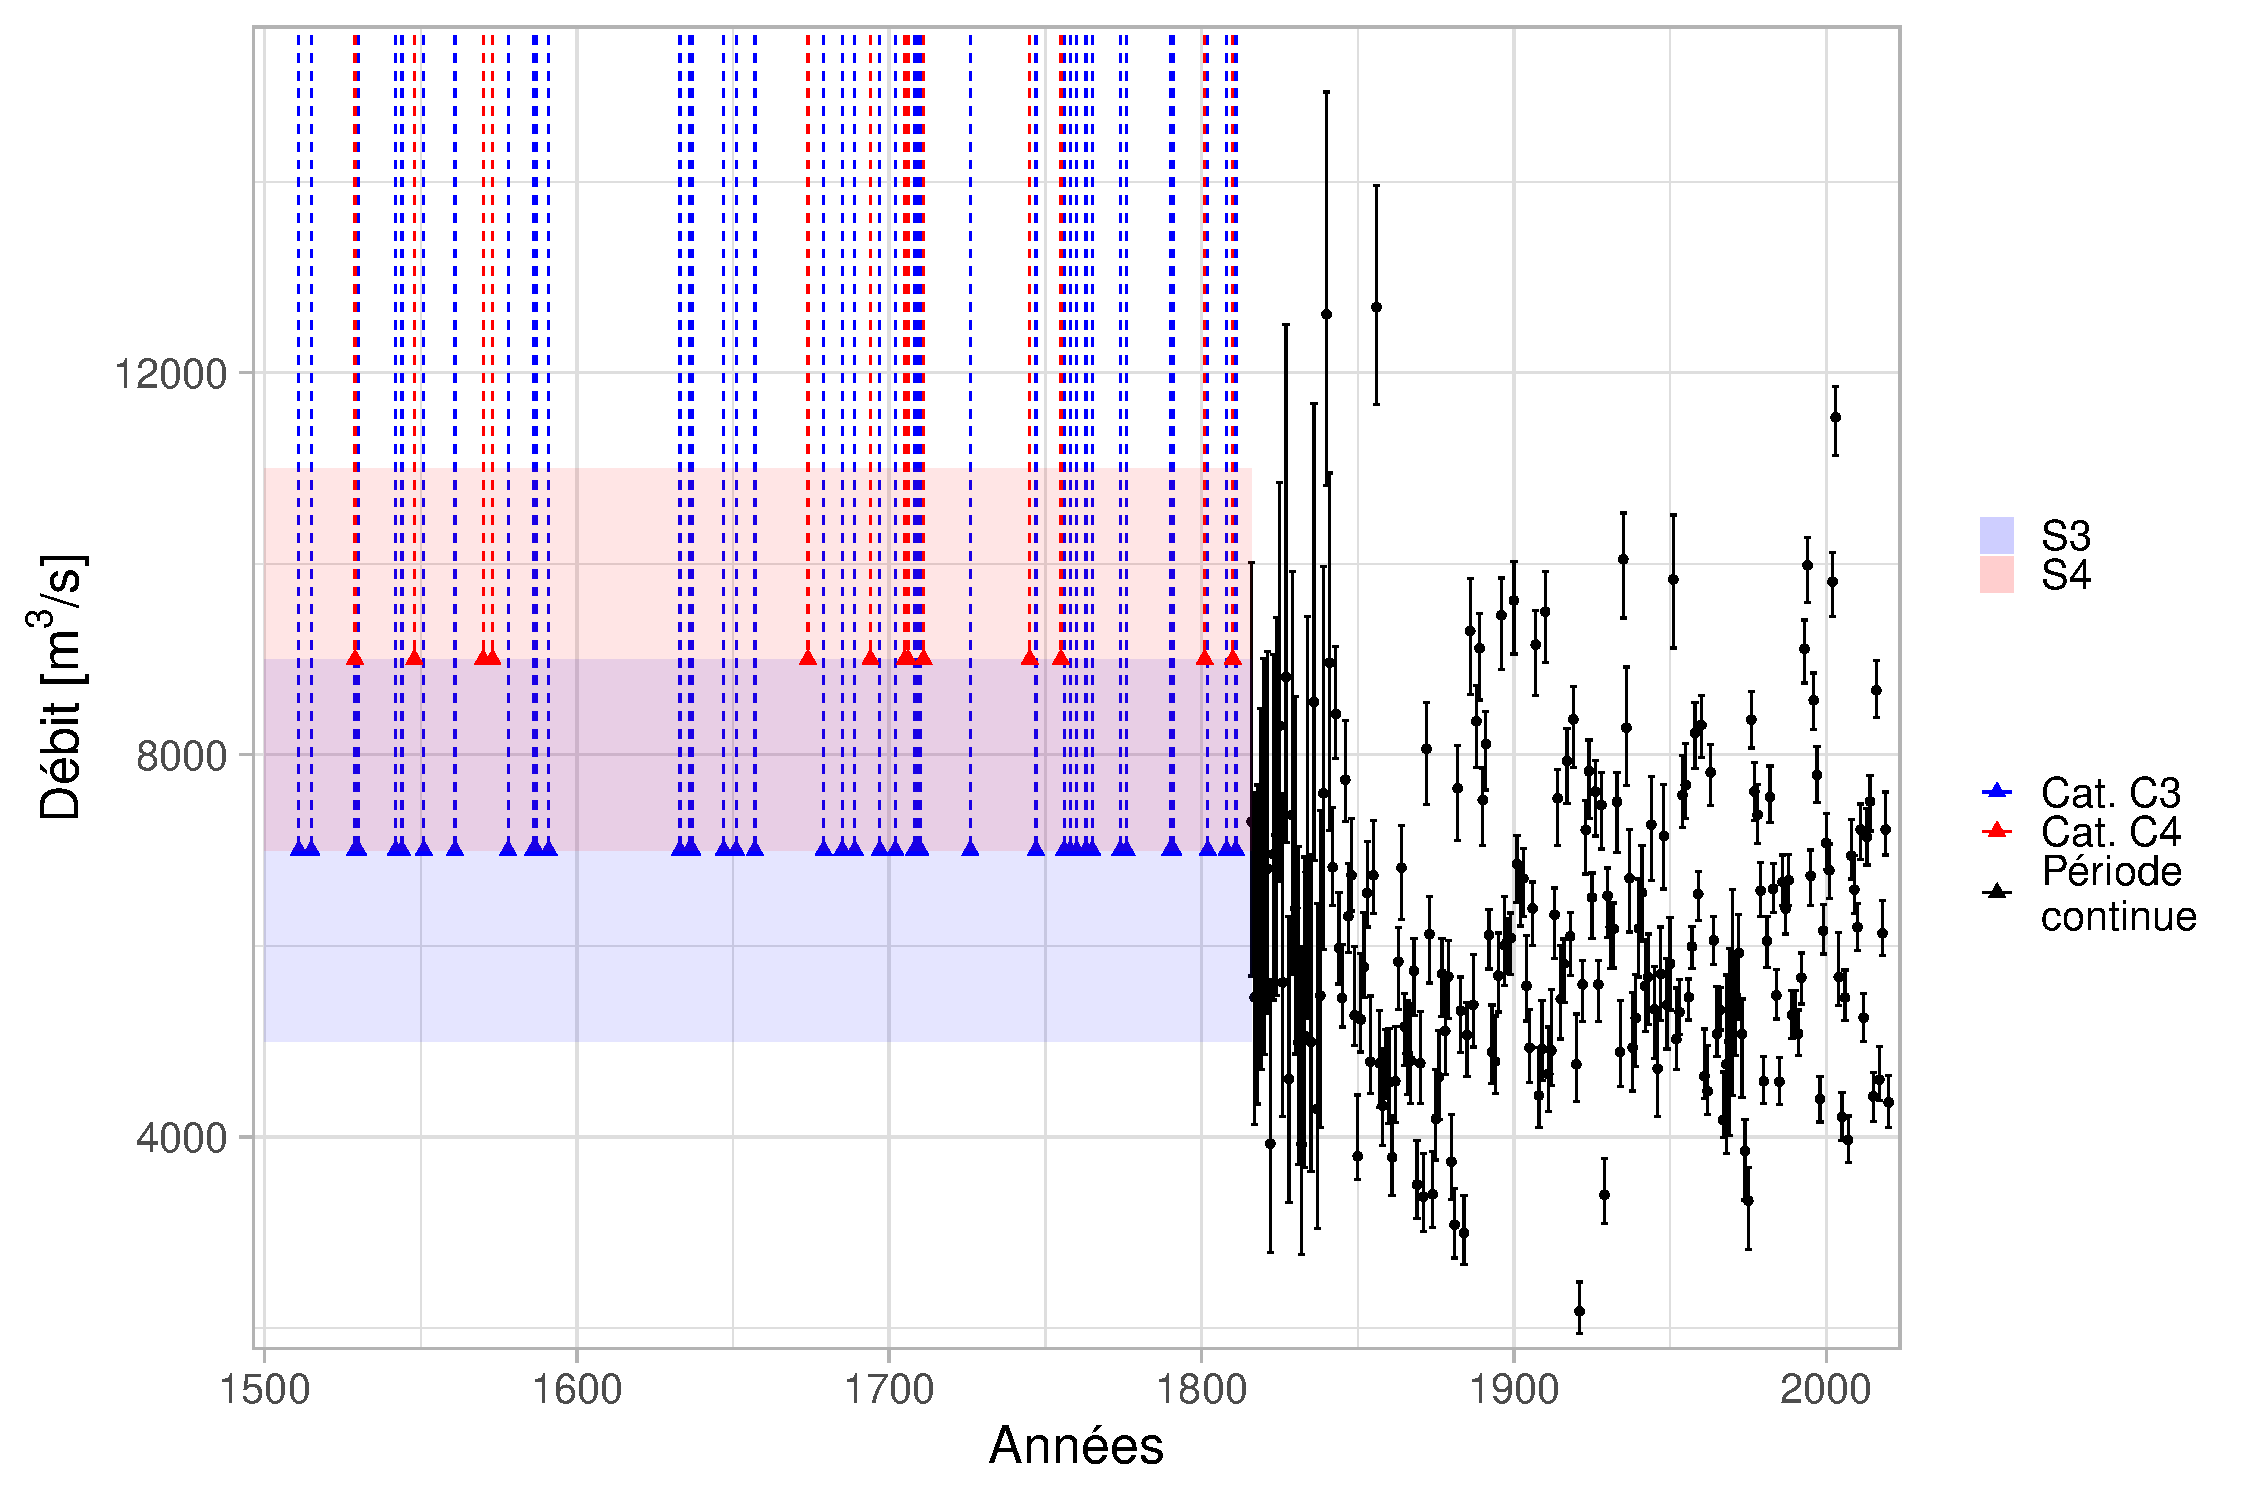
\includegraphics[width=.9\linewidth]{Figures/EchMixteBcr.pdf}	
		\caption{Échantillon de crues du Rhône à Beaucaire. L'incertitude autour des seuils de perception est représentée par les bandeaux bleus et rouge ("S3" et "S4)}
		\label{fig:EchMixte}
	\end{figure}
	

	\subsection{Homogénéité des données}
	\paragraph{} L'homogénéité des données est un pré-requis essentiel à l'analyse fréquentielle des crues en contexte stationnaire, car cette dernière repose sur l'hypothèse que les variables étudiées sont dites $iid$ (indépendantes et identiquement distribuées). C'est à dire que les processus statistiques pouvant être utilisés pour modéliser la distribution des crues ne changent pas dans le temps, et que pour une station donnée, une même distribution peut être utilisée pour modéliser les crues du XIX\textsuperscript{ème} et du XXI\textsuperscript{ème} siècle. Étant donné que deux types d'échantillons sont utilisés, deux types de tests statistiques sont utilisés pour étudier l'homogénéité de ces échantillons. 

	\subsubsection{Données continues}
	
	\paragraph{} Deux tests seront utilisés pour qualifier l'homogénéité de l'échantillon de données continues : le test de Pettitt (REF) et le test de Mann-Kendall (REF). Ils permettent de détecter deux formes de non-homogénéités de la distribution séries temporelles : les ruptures et les tendances. Les ruptures sont des changements soudains (i.e. les données ont une distribution différente avant et après un instant $t$), tandis les tendances représentent des changements progressifs dans la distribution des données au cours du temps. L'incertitude autour des débits maximum annuels à Beaucaire a été déterminée au Chapitre 1 (REF) et est représentée par 500 réalisations possibles de la série temporelle. Cette incertitude étant propagée aux estimations des quantiles de crue, il est nécessaire d'appliquer les tests à l'ensemble des réalisations.
	\paragraph{} Au risque d'erreur 5\%, le test de Pettitt a conclu à l'existence d'une rupture pour 60\% des 500 réalisations testés. ET DONC ?
	
	\paragraph{} L'application du test de Mann-Kendall a permis de conclure que seulement 20\% des 500 réalisations de débits maximum annuels comportent une tendance temporelle. ET DONC ?
	
	\paragraph{} L'échantillon de données continues peut être considéré homogène suite aux tests statistiques réalisés. 
	
		
	\subsubsection{Données historiques}
	
	\paragraph{} Les données pré-enregistrements continus sont ici utilisés comme étant des occurrences de crues supposées supérieures à un seuil. Comme décrit par \citet{lang_towards_1999}, la fréquence des occurrences de crues sup-seuil est supposée suivre un processus de Poisson. Afin de vérifier l'homogénéité des occurrences sup-seuil, il est possible de calculer un intervalle de confiance autour du nombre cumulé de crues découlant du processus de Poisson. Si les occurrences de crues cumulées "sortent" de cet intervalle de confiance, alors leur fréquence d'occurrence est supposée non-stationnaire. 
	
	\paragraph{} Ces intervalles de confiance ont été calculés pour l'échantillon de crues pré-enregistrements continus du Rhône à Beaucaire. Le début de la période historique est supposé débuter en 1500 et se termine à l'année des premiers enregistrements continus de hauteur d'eau, en 1816. Les deux échantillons testés ici reflètent deux seuils de perception, $S3$ et $S4$, et on a $S3 > S4$. 

	\begin{figure}[h]
		\centering
		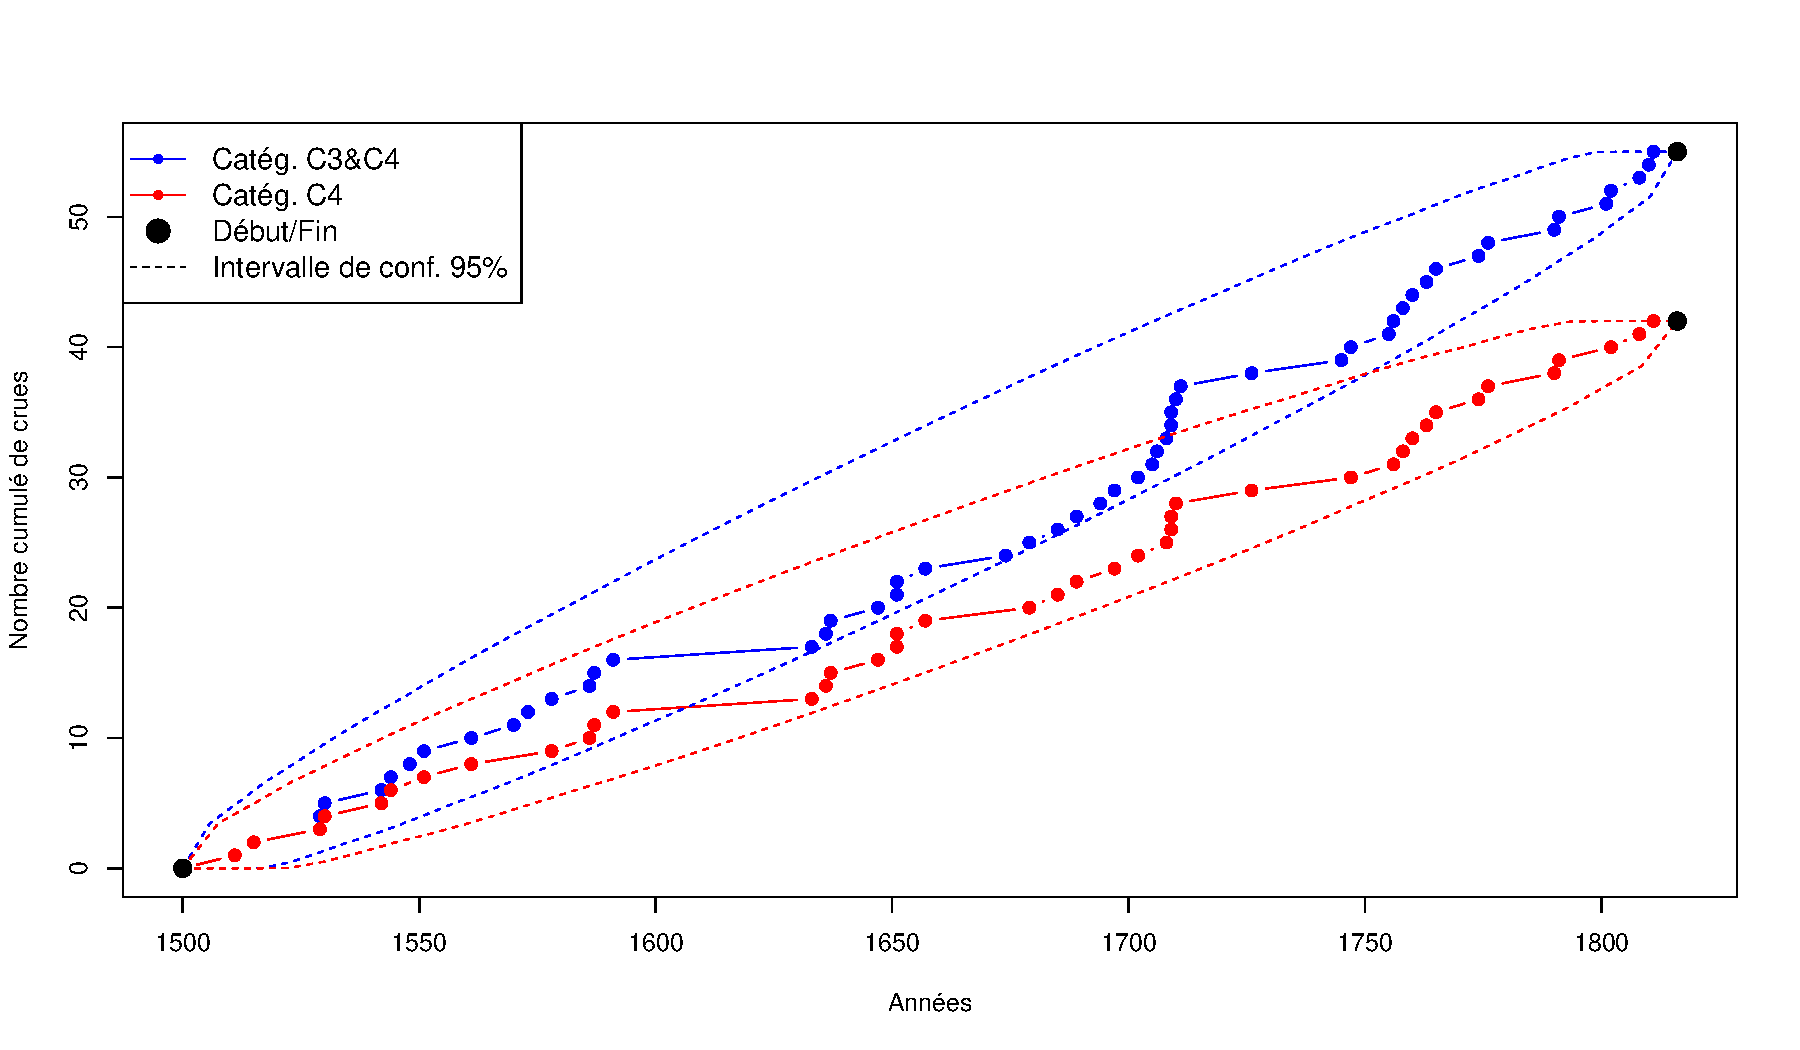
\includegraphics[width=.8\linewidth]{Figures/Poisson_C3-C4_FR.pdf}	
		\caption{Nombre de crues cumulé et intervalles de confiance à 95\% du processus de 						Poisson, pour deux échantillons d'occurrences de crues sup-seuil à Beaucaire 							(1500-1816)}
		\label{fig:Poisson_C3-C4}
	\end{figure}		
	
	\paragraph{} Sur la figure \ref{fig:Poisson_C3-C4}, on remarque que les nombre cumulés de crues des deux échantillons ne sortent pas des intervalles de confiance à 95\%, ils sont donc tous les deux homogènes. L'échantillon correspondant au seuil $S3$ (en bleu) se rapproche de la borne inférieure de l'intervalle de confiance au XVII\textsuperscript{ème} siècle, mais revient rapidement dans des valeurs moyennes à la faveur de nombreuses crues sup-seuil au début du XVIII\textsuperscript{ème} siècle. 
	
	\paragraph{} L'échantillon continu de débits maximum annuels (1816-2020) sera par la suite artificiellement "dégradé" pour reproduire des durées de chroniques plus usuelles. Ainsi, les crues dont le débit maxpost est supérieur au seuil considéré sont retenues dans l'échantillon. Cette période "dégradée" commence au début de la chronique, en 1816, et se termine en 1970, à la mise en fonctionnement de la station de Beaucaire Restitution. Deux seuils de perception similaires aux seuils $S3$ et $S4$ sont ici étudiés : 7000 et 9000 $m^3/s$. L'homogénéité de ces deux échantillons "artificiels" est testée dans la figure \ref{fig:Poisson_Recent}. Les deux échantillons de crues cumulés ne sortent pas des intervalles confiance à 95\%, ils sont donc tous deux homogènes. 
	
	\begin{figure}[h]
		\centering
		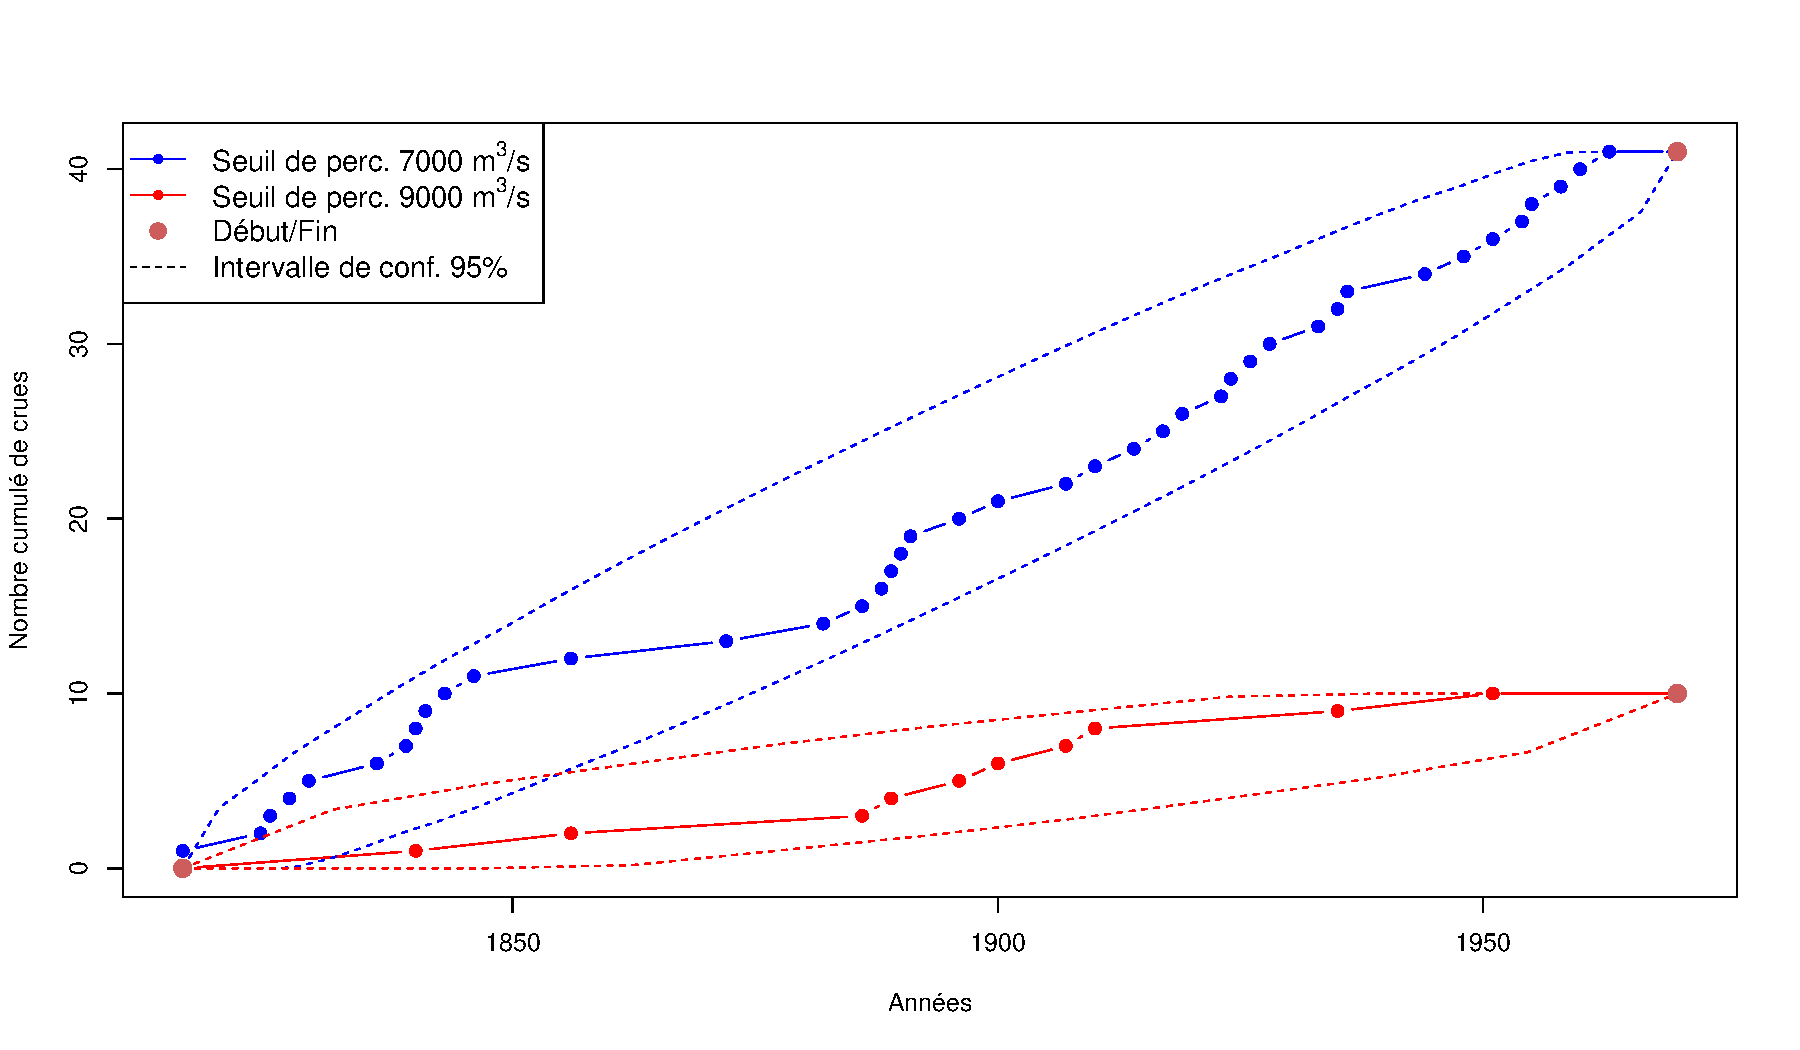
\includegraphics[width=.8\linewidth]{Figures/Poisson_Qrecent_FR.pdf}	
		\caption{Nombre de crues cumulé et intervalles de confiance à 95\% du processus de 						Poisson, pour deux échantillons d'occurrences de crues sup-seuil à Pont de Beaucaire 							(1816-1969)}
		\label{fig:Poisson_Recent}
	\end{figure}
	
	
		
\FloatBarrier		
	
	
\section{Application aux crues du Rhône à Beaucaire}

	\paragraph{}
	Les 4 modèles décrits dans les sections précédentes (A, B, C et D) sont appliqués aux 4 échantillons de crues du Rhône à Beaucaire présentés dans le tableau \ref{tab:Echantillons}. Les échantillons 1 et 2 sont basés sur les débits estimés au chapitre 1(REF) qui ont été dégradés pour créer artificiellement un échantillon mixte de données continues (1970-2020) et ponctuelles (1816-1969). Il s'agit ici de tailles d'échantillon plus usuelles et dont le seuil de perception et la durée de la période historique sont parfaitement connus, contrairement aux échantillons 3 et 4. Ainsi, pour les modèles faisant l'hypothèse que le seuil de perception et/ou la durée de la période historique sont inconnus, on jugera notamment la capacité du modèle à converger vers des valeurs acceptables. 
	
	\begin{table}[h]
		\centering
		\resizebox{\linewidth}{!}{%
		\begin{tabular}{|m{0.03\textwidth}
						|m{0.13\textwidth}
						|m{0.1\textwidth}
						|m{0.1\textwidth}
						|m{0.1\textwidth}
						|m{0.1\textwidth}
						|m{0.12\textwidth}
						|m{0.14\textwidth}
						|m{0.12\textwidth}
						|m{0.14\textwidth}|}
		\hline
		  n° & 
		  Échantillon &
		  Période historique &
		  Nb. sup-seuil histo. &
		  Période continue &
		  Nb. sup-seuil cont. &
		  Seuil de percep. [$m^3/s$] &
		  A priori seuil [$m^3/s$]  &
		  Date de début histo. &
		  A priori date début histo. \\ \hline
		1 & 1816-2020 dégradé $S3$ & 1816-1969 & 41 & 1970-2020 & 16 & 7000 & $\mathcal{N}(7000,2000)$ & 1816 & $\mathcal{U}(1816,1316)$ \\ \hline
		2 & 1816-2020 dégradé $S4$ & 1816-1969 & 10 & 1970-2020 & 4 & 9000 & $\mathcal{N}(9000,2000)$ & 1816 & $\mathcal{U}(1840,1340)$\\ \hline
		3 & 1500-2020 $S3$ & 1500-1815 & 55 & 1816-2020 & 57 & 7000 & $\mathcal{N}(7000,2000)$ & 1500 & $\mathcal{U}(1511,1111)$\\ \hline
		4 & 1500-2020 $S4$ & 1500-1815 & 13 & 1816-2020 & 14 & 9000 & $\mathcal{N}(9000,2000)$ & 1500 & $\mathcal{U}(1529,1129)$\\ \hline
		\end{tabular}%
		}
		\caption{Échantillons de crues du Rhône à Beaucaire}
		\label{tab:Echantillons}
	\end{table}
	
	Pour les modèles qui font l'hypothèse d'un seuil de perception connu (A et C), le seuil retenu est présenté dans le tableau. Il en est de même pour les modèles qui font l'hypothèse d'une durée de période historique connue (B et D). Ici, par souci de clarté, ce n'est pas la durée de la période historique $n$ qui sera examinée mais la date de début de la période historique. Lorsque cette date est supposée méconnue, l'a priori débute à la date de la première crue de l'échantillon.
			
	\FloatBarrier	
	
	\subsection{Résultats pour la période récente dégradée (1816-2020)}
	
	\paragraph{} 
	
	UNIQUEMENT ARTIF 2? 
	
	\subsubsection{BASELINE(S) VS A : quel est l'apport des crues historiques pour une longueur de chronique "courante" ?}

\begin{figure}[h]
        \centering
        \begin{subfigure}{.8\textwidth}
                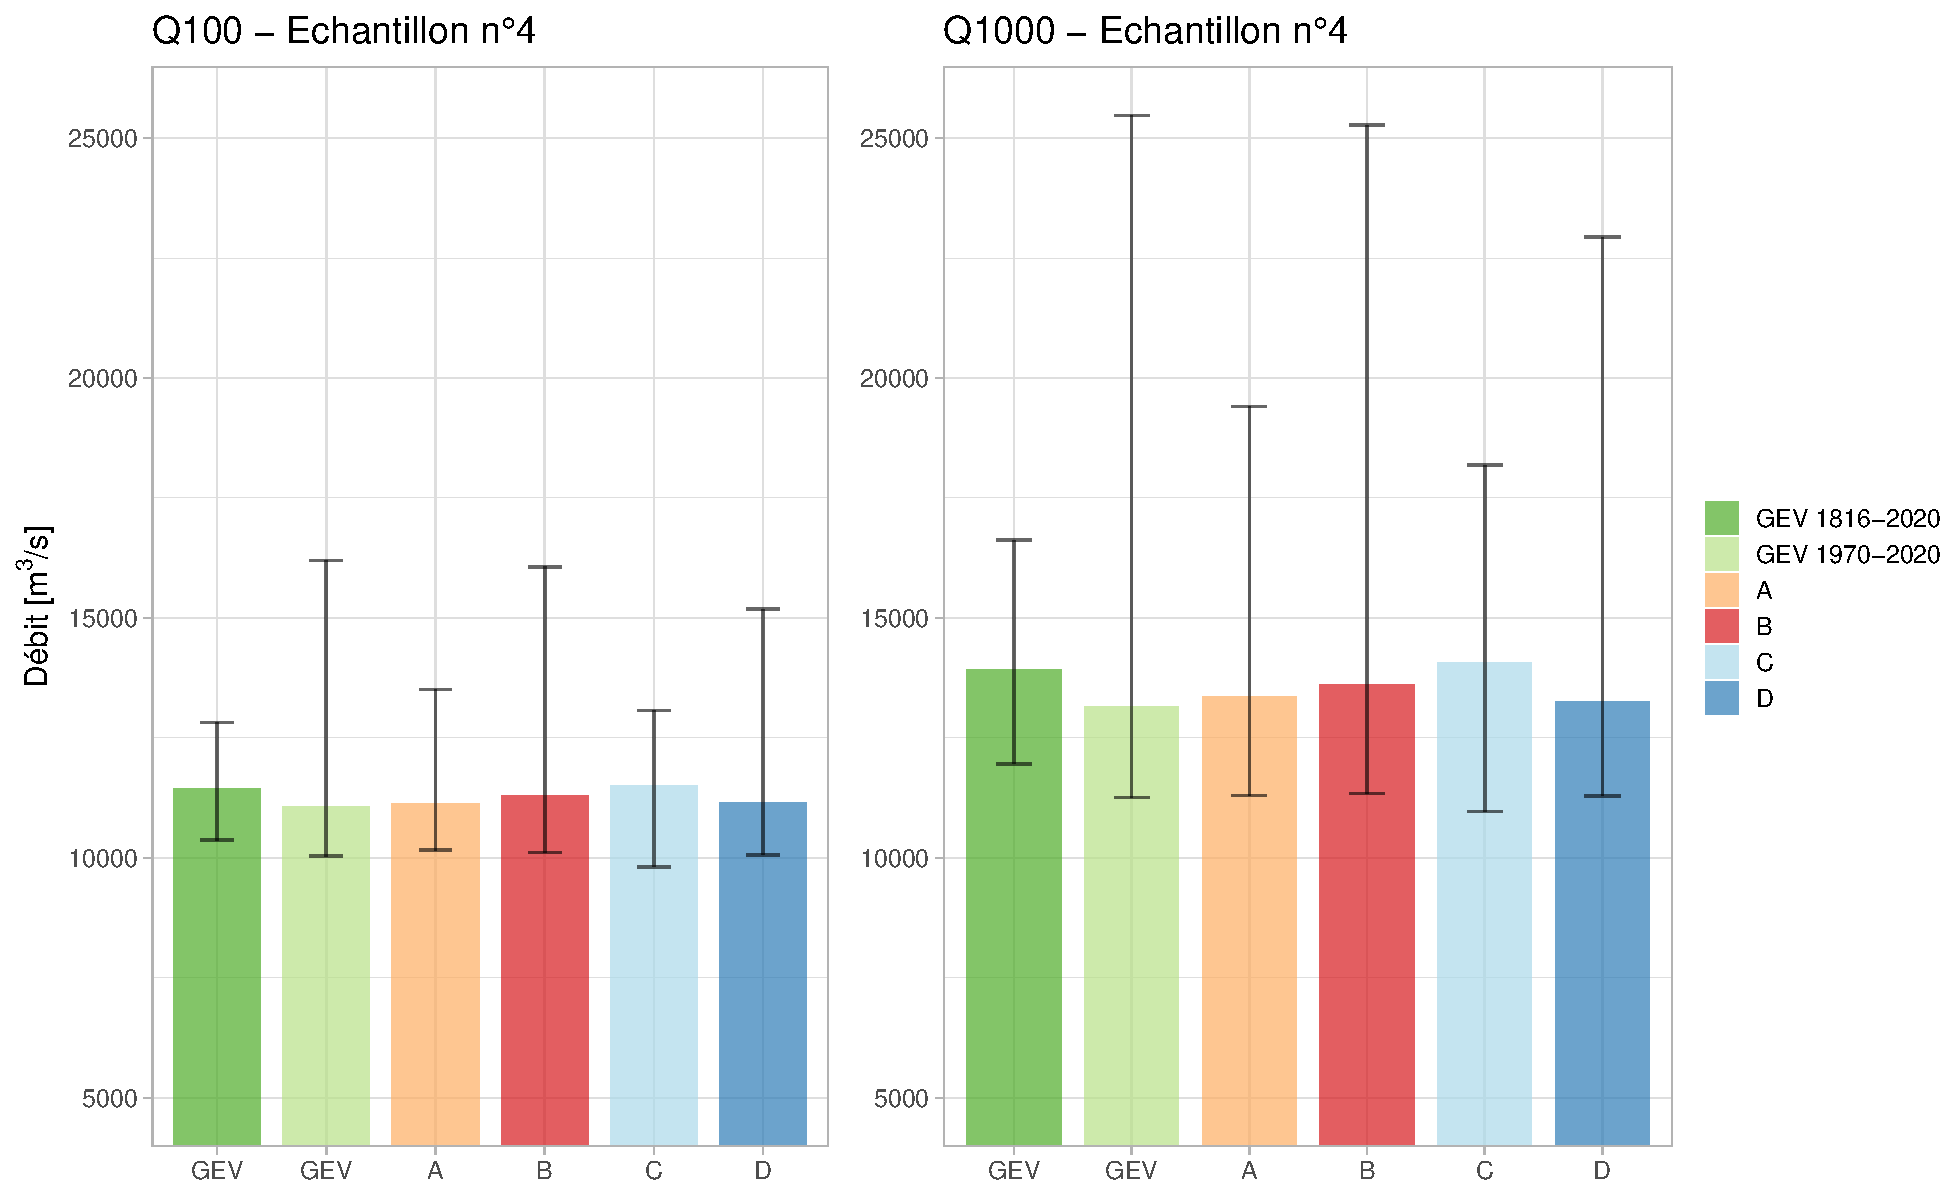
\includegraphics[width=.8\textwidth]{Figures/Barplots_QX_Artif2.pdf}
                \caption{}
                \label{subfig:Barplot_Artif2}
        \end{subfigure}
        \centering
        \begin{subfigure}{\textwidth}
                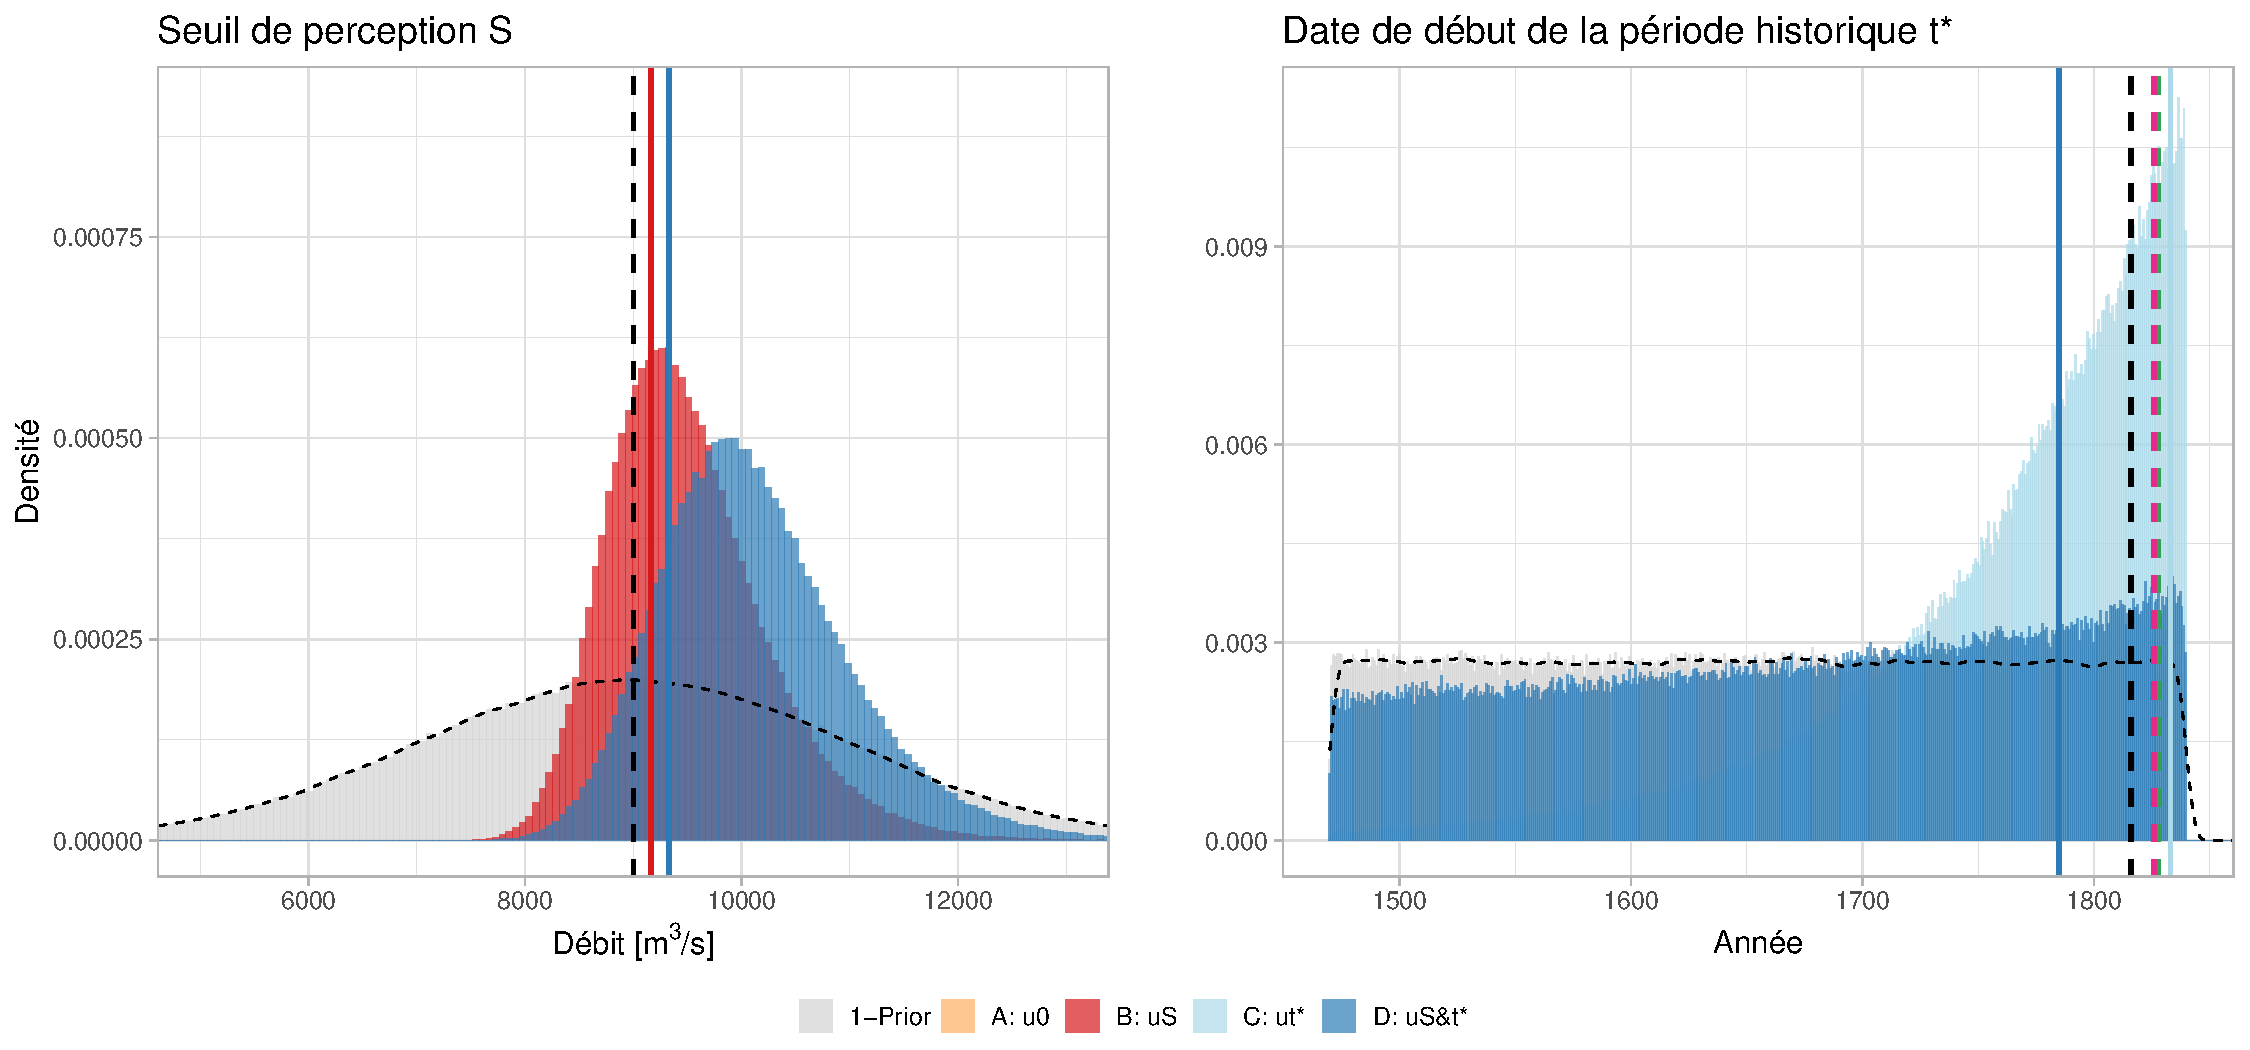
\includegraphics[width=.8\textwidth]{Figures/Params_Artif2.pdf}
                \caption{}
                \label{subfig:Params_Artif2}
        \end{subfigure}
        \caption{(a) Barplot des estimations de débit des périodes de retour 100 et 1000 ans pour 6 modèles. Basé sur les crues supérieures à un seuil de 9000 $m^3/s$ de 1816 à 1969 et les débits max annuels de 1970 à 2020 à Beaucaire. (b) Estimations a posteriori de trois des paramètres. Les a priori sont affichés en gris.}
\end{figure}

	\paragraph{} Dans la figure \ref{subfig:Barplot_Artif2}, les résultats du modèle mixte sont comparés aux résultats du modèle présenté au Chapitre 1 (REF) (ici appelé GEV) pour les débits maximum annuels de 1816 à 2020 et de 1970 à 2020. On remarque dans un premier temps que l'incertitude autour de l'estimation de la crue millénale pour le modèle GEV 1970-2020 est très importante, ce qui souligne l'intérêt de valoriser les crues historiques lorsque les données continues disponibles couvrent une période trop courte (ici 50 ans). 
	\paragraph{} Les estimations maxpost des modèles mixtes (i.e. GEV et Binomiale) sont relativement proches de la référence (GEV 1816-2020). En revanche, les enveloppes d'incertitudes sont de taille très variables en fonction du modèle, particulièrement pour les estimations millénales. Les résultats des modèles A et C ont des incertitudes comparables et qui semblent acceptables (VALEURS EN \%?). Le fait de supposer seulement la durée de la période historique comme étant inconnue semble donc peu impactant sur l'incertitude du résultat. En revanche, lorsque le seuil devient inconnu (B et D), la largeur de l'intervalle de confiance est quasiment multiplié par deux. 
	\paragraph{} Les paramètres a posteriori sont présentés dans la figure \ref{subfig:Params_Artif2}. Les paramètres de forme estimés sont tous proches de la référence, soit légèrement positifs. Pour le seuil de perception dont la vraie valeur est ici 9000 $m^3/s$, les estimations maxpost pour les modèles B et D sont respectivement de 9163 et 9331 $m^3/s$. Le modèle converge donc vers des valeurs très proches. En revanche, la distribution pour le modèle D semble décalée vers des valeurs plus fortes, probablement pour compenser l'estimation d'une durée de période historique trop longue. Sur le graphique de droite, la durée de la période historique est présentée sous la forme de la date de début de la période dont la vraie valeur est ici est l'année 1816. L'a  priori étant une distribution uniforme qui débute à l'année de la première crue de l'échantillon (ici en 1840), il est possible de trouver des dates plus anciennes ou plus récentes que la vraie valeur. La période historique estimée par le modèle C débute en 1833, elle est donc plus courte que la réalité. En revanche, le modèle D estime un début de période maxpost en 1785. La distribution des durées de période du modèle C semble bien plus raisonnable que celle du modèle D, pour lequel la densité est pratiquement uniforme et donc très proche de l'a priori (qui pour cette raison n'est pas visible ici). Sans surprise, une méconnaissance du seuil et de la durée de la période historique complexifie l'estimation des paramètres. Quand un seul des deux est méconnu, les paramètres sont en revanche bien mieux estimés. Il faut aussi noter que ces résultats sont dépendants du choix du seuil de perception "artificiel", fixé ici à 9000 $m^3/s$ (il est dépassé par 10 crues entre 1816 et 1970).
	\\
	Les résultats pourraient être différents pour un autre seuil, monter A artif1 VS A artif 2? \\
	(AJOUTER LE SCATTERPLOT POUR LE MODELE D?)\\
	(GRAPHE DES QUANTILES?)\\
	
	\begin{figure}[h]
        \centering
        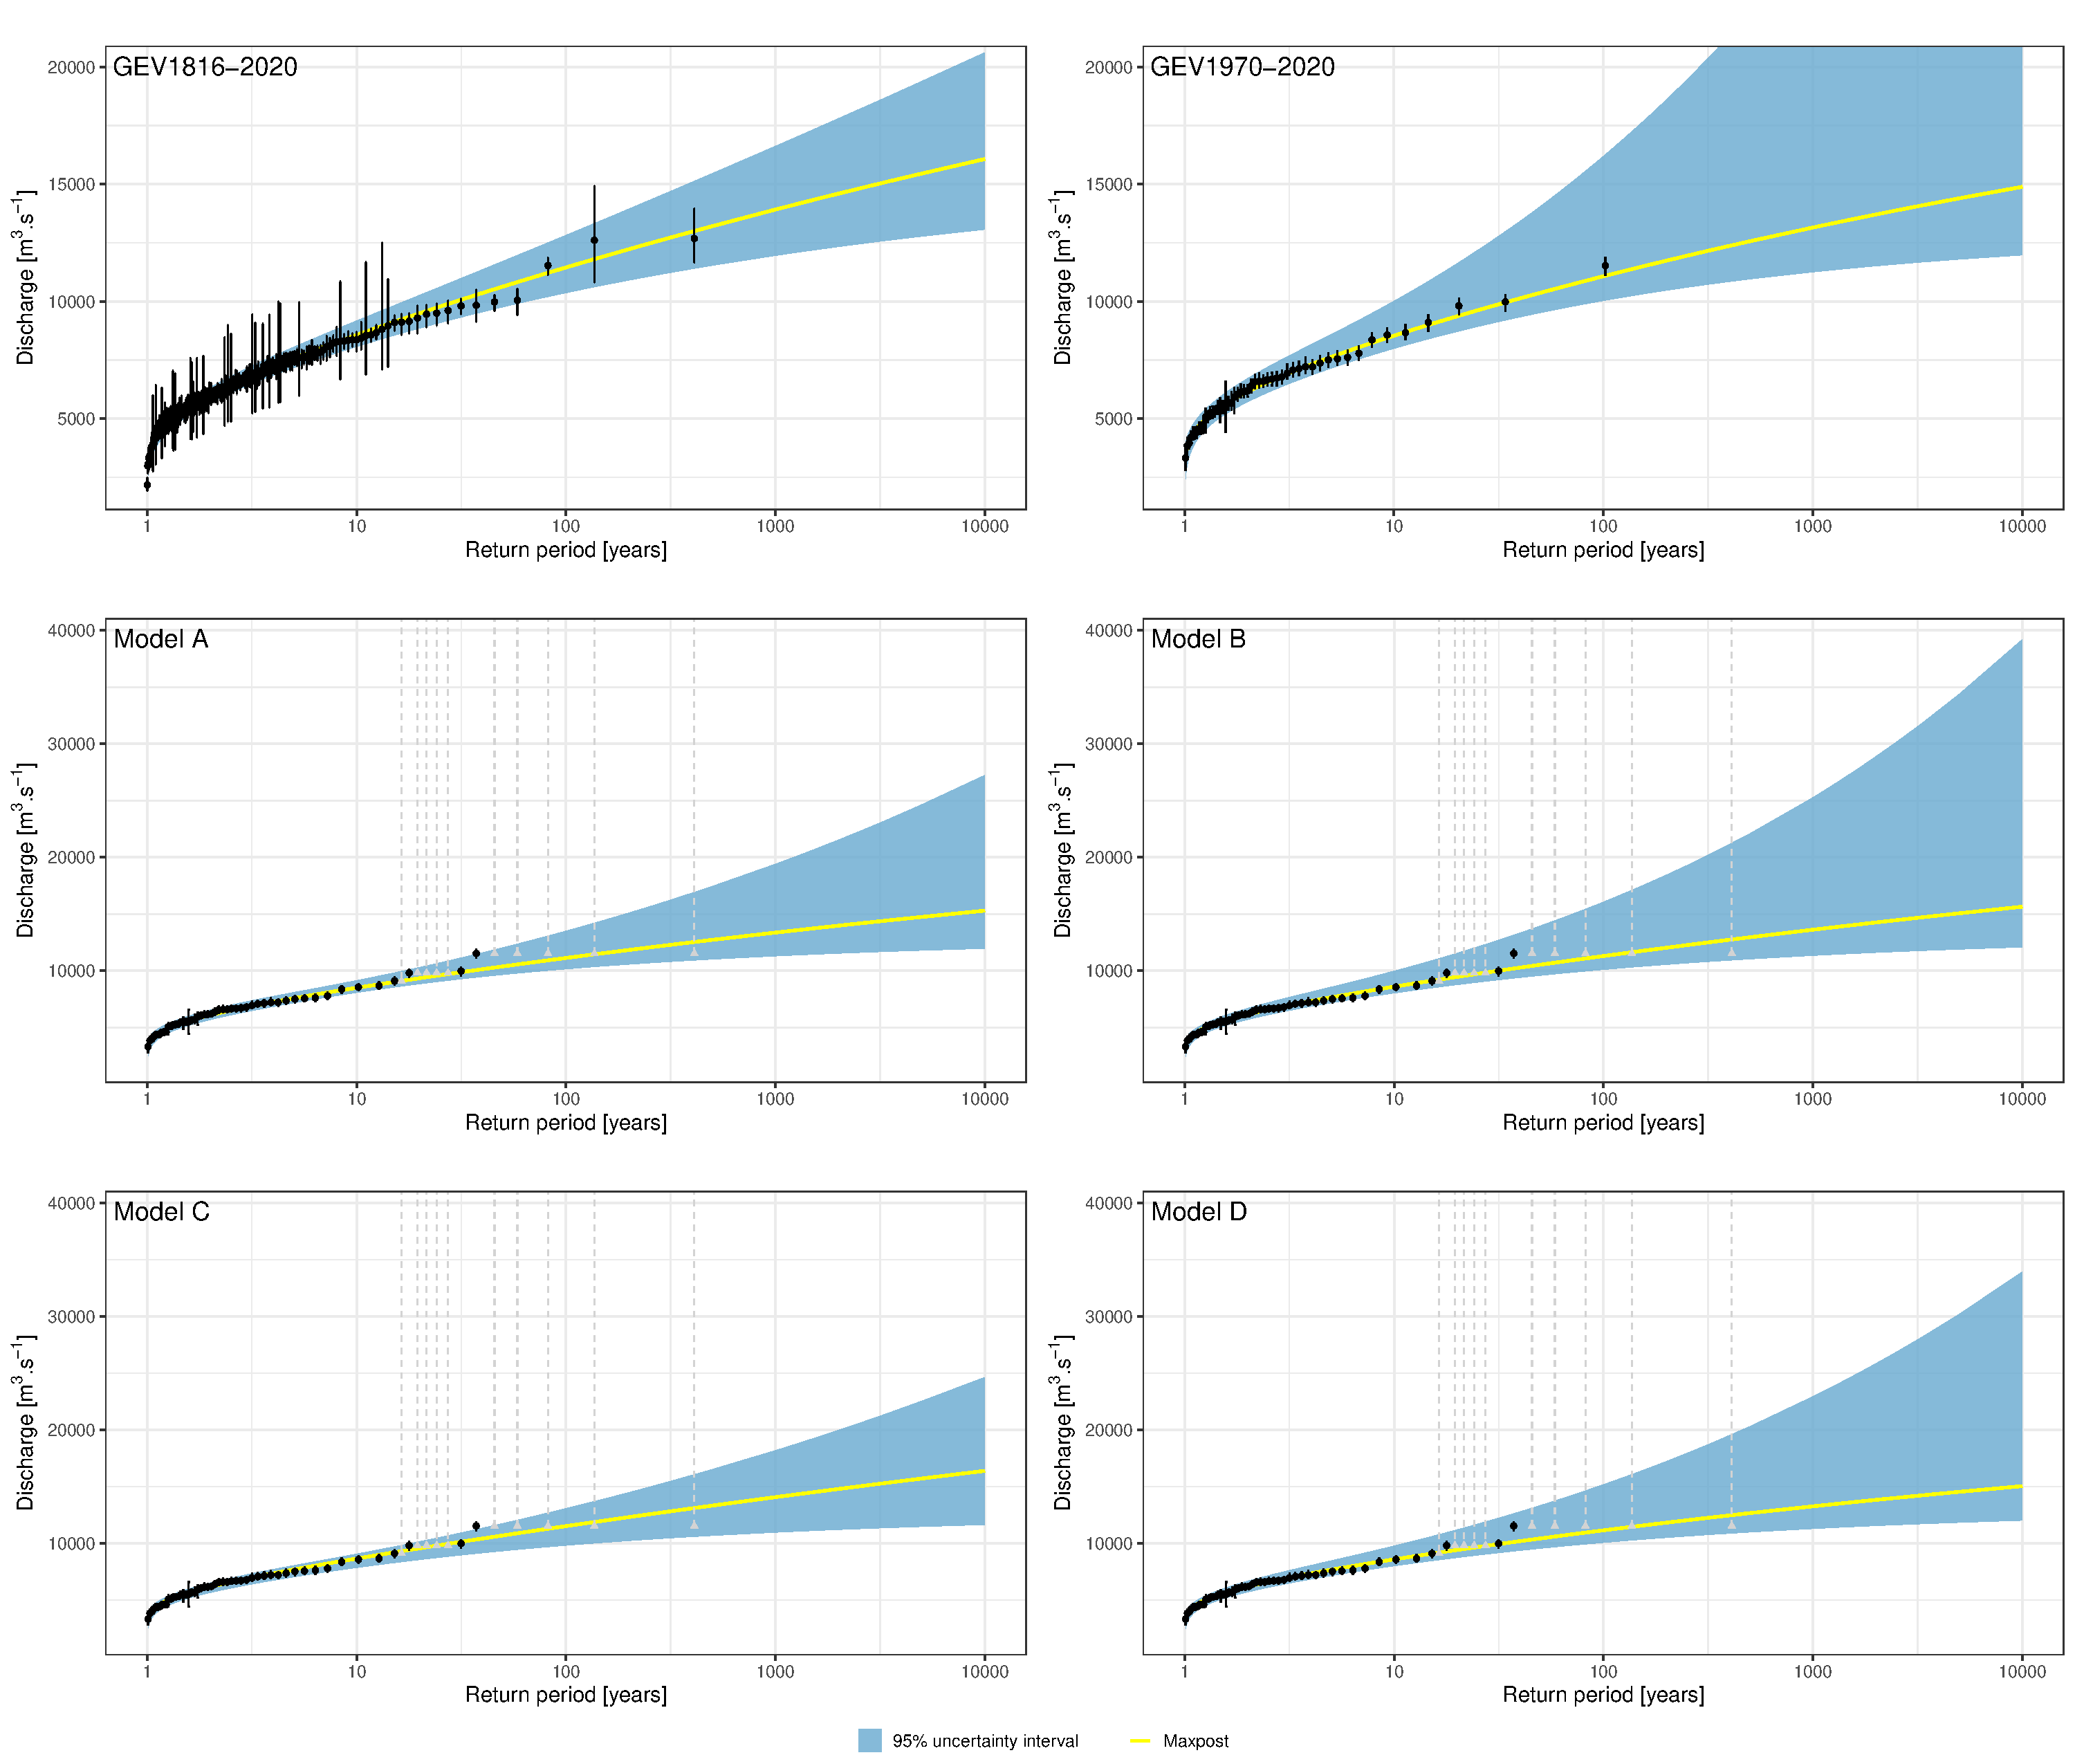
\includegraphics[width=.9\linewidth]{Figures/Quantiles_Artif2.pdf}
        \caption{Quantiles estimés sur l'échantillon 2 pour les 6 modèles. Les crues de la période continue sont en noir, les crues de la période historiques en gris}
        \label{fig:Quants_Artif2}
\end{figure}
		
\FloatBarrier


		\subsubsection{BASELINE(S) VS A VS B : quel est l'impact de la méconnaissance du seuil de perception ?}
	
		IC A vs B + est-ce que le modèle converge vers le vrai seuil ? 
		ARTIF 2 uniquement ? 
		
		\subsubsection{BASELINE(S) VS A VS C : quel est l'impact de la méconnaissance de la durée de la période historique ?}
	
		IC A vs C + est-ce que le modèle converge vers la vraie durée ? 
		ARTIF 2 uniquement ? 
		
		\subsubsection{BASELINE(S) VS A VS D : quel est l'impact de la méconnaissance de la durée de la période historique ET du seuil de perception?}
	
	\subsection{Application à la période 1500-2020}

	
		\subsubsection{BASELINE VS A pour l'échantillon C3?. Quel est l'apport des crues historiques pour l'analyse fréquentielle à Beaucaire ?}
	Comparaison des résultats du modèle (Baseline) avec les résultats du modèle (A) pour l'échantillon ("C3 et C4").\\
	Barplot Q100 et Q1000
	
		\subsubsection{Modèle A pour les échantillons C3+C4 VS C4 : Quel est l'impact du choix de l'échantillon de crues historiques ("C3etC4" vs "C4")}
	Comparaison des résultats du modèle (A) pour les échantillon ("C3 \& C4") et ("C4")\\
	Barplot Q100 et Q1000	
	
		\subsubsection{Quel est l'impact de la méconnaissance du seuil de perception ?}
	Comparaison des résultats du modèle (A) et du modèle (B) pour l'échantillon ("C3 \& C4")\\
	Barplot Q100 et Q1000, et comparaison de la distribution a postériori du seuil
	
		\subsubsection{Quel est l'impact de la méconnaissance de la durée de la période historique ?}
	
	Comparaison des résultats du modèle (B) et du modèle (C) pour l'échantillon ("C3 \& C4")\\
	Barplot Q100 et Q1000, comparaison de la distribution a postériori du seuil et de la taille de la période historique\\
	Comparaison de la date de début de la période historique estimée par le modèle (maxpost) avec la date obtenue via la méthode de \cite{prosdocimi_german_2018}.\\

	
	\subsection{Discussion}
	
\section{Conclusion du chapitre}
	Conclusions sur l'intérêt des crues historique pour l'estimation des quantiles extrêmes à Beaucaire. \\
	Est-ce qu'on observe une réelle amélioration avec les résultats du chapitre 1 ?\\
	Selon les résultats, ajouter quelque chose comme : "l'utilisation des crues historiques peut mener à faire de fortes hypothèses (seuil et durée de la période), il faut être pragmatique sur la considération des incertitudes\\
	Ces conclusions sont valables uniquement à Beaucaire (période continue très longue, paramètre de forme positif, pas de tendance observée due au changement climatique ou autre). Mais que nous à appris l'application du modèle à un échantillon dégradé plus représentatif des longueurs de chronique habituelles ?\\
	Perspectives sur les modèles d'analyse fréquentielle en contexte non-stationnaire et sur les modèles régionaux.  

\printbibliography
\end{document}
